\documentclass[14pt]{beamer}
\usepackage[utf8]{inputenc}
\usepackage[T1]{fontenc}
\usepackage{lmodern}
\usepackage[english]{babel}
\usepackage{amsmath}
\usepackage{amsfonts}
\usepackage{amssymb}
\usepackage{graphicx}
\usetheme{AnnArbor}

\newcommand\e{\emph}
\newcommand\tb{\textbf}
\newcommand\un{\underline}
\newcommand\txt{\texttt}

\AtBeginSection[]{
	\begin{frame}
	\vfill
	\centering
	\begin{beamercolorbox}[sep=8pt,center,shadow=true,rounded=true]{title}
		\usebeamerfont{title}\insertsectionhead\par%
	\end{beamercolorbox}
	\vfill
\end{frame}
}


\begin{document}
\author[Lin, J., and Graham, S.] % (optional)
{Jennifer Lin\inst{1} and Steven Graham\inst{2}}
	\title{Will God’s Grace Guide My Vote?}
	%\subtitle{}
	%\logo{}
	\institute[]{	
		\inst{1}%
		Undergraduate Student\\
		New College of Florida
		\and
		\inst{2}%
		Faculty of Psychology\\
		New College of Florida}
		
	\date[FPSA 2019]{Florida Political Science Association, March 2019}
	%\subject{New College of Florida}
	\setbeamercovered{transparent}
	\setbeamertemplate{navigation symbols}{}
	\begin{frame}[plain]
	\maketitle
\end{frame}

\begin{frame}
\frametitle{Guiding Questions}
\begin{enumerate}
	\item Do subliminal religious primes influence political decision-making?
	\item If yes, in which direction on the left-right scale?
\end{enumerate}
\end{frame}

\begin{frame}
\frametitle{Past Research}
\begin{itemize}
	\item Religion is a central aspect to American life
	\item Personal identities shape political decision-making processes
	\item Past research suggests that individuals who vote in churches, or who are otherwise reminded of their religiosity, tend to be more conservative
\end{itemize}
\end{frame}

\begin{frame}
\frametitle{Hypotheses}
\begin{enumerate}
	\item Religious primes influence political decisions
	\item People think more conservatively in the religious mindset
\end{enumerate}
\end{frame}

\section{Experimental Method}

\begin{frame}
\frametitle{Participants}
\begin{itemize}
	\item 296 of 356 original respondents incorporated in analysis (126 identify as female)
	\item Recruited via Amazon Mechanical Turk
	\item Participants were paid \$ 1 for their participation
\end{itemize}
\end{frame}

\begin{frame}
\frametitle{Procedure}
\begin{itemize}
	\item Sentence Reorganization
	\item Statement and Agreement on Controversial Issue
	\item Religiosity Measure
	\item Demographic Questions
	\item Manipulation Check
\end{itemize}
\end{frame}

\section{Results}

\begin{frame}
\frametitle{Method of Analysis}
\begin{itemize}
	\item 2 (Prime Condition) $\times$ 2 (Issue Condition) ANOVA
	\item $\alpha = .05$
\end{itemize}
\end{frame}

\begin{frame}
\frametitle{Results}
\begin{table}
	\centering
	\small
	\begin{tabular}{lccccc}
		\hline
		\tb{Variables}&\tb{df}&\tb{SS}&\tb{MS}&\tb{F}&\tb{p-value}\\
		\hline
		Prime Condition&1&0.00&0.00&0.00&0.984\\
		Argument Condition&1&280.00&280.03&56.22&0.001***\\
		Interaction&1&0.8&0.79&0.159&0.690\\
		\hline
	\end{tabular}\\
Note: * p$<$0.05; ** p$<$0.01; *** p$<$0.001
\end{table}
\end{frame}

\begin{frame}
\frametitle{Interaction Plot}
\begin{figure}
	\centering
	{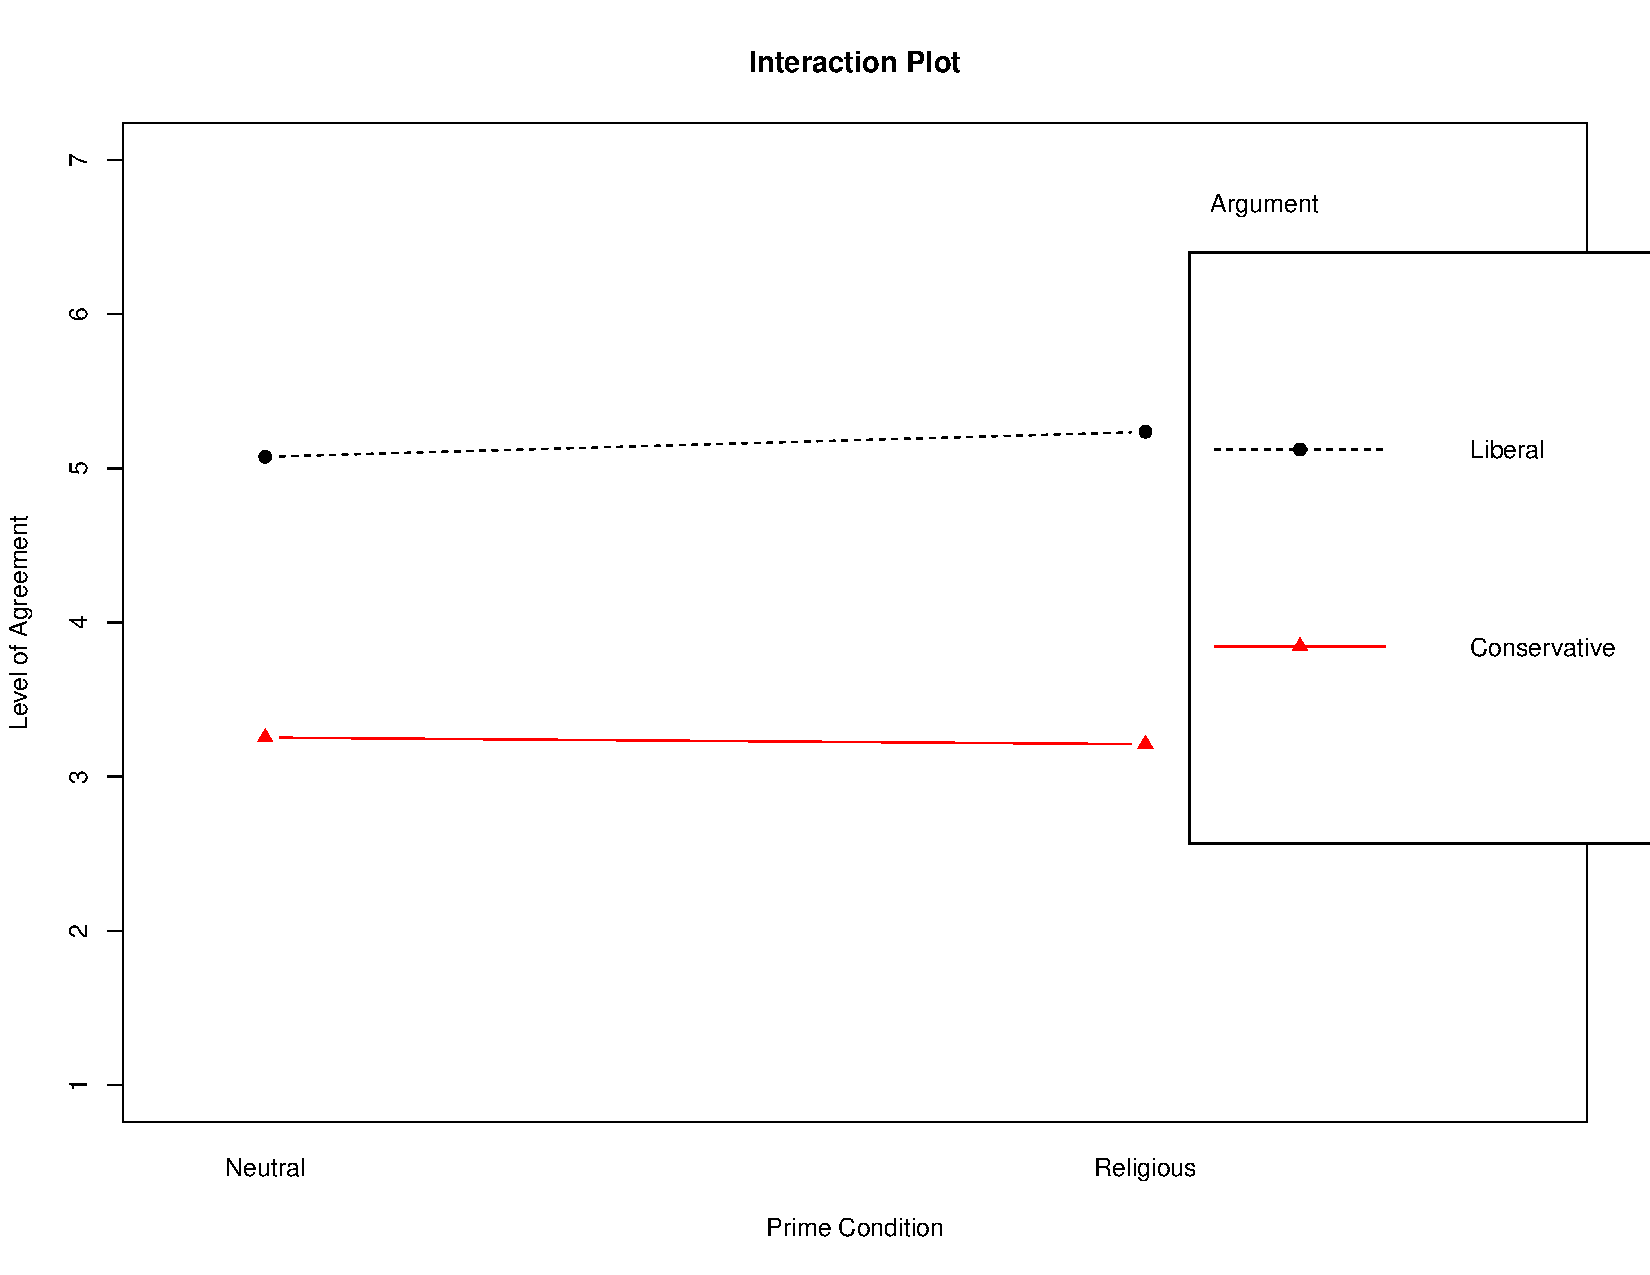
\includegraphics[width=.8\textwidth]{InteractionPlot}}
\end{figure}
\end{frame}

\section{General Discussion}

\begin{frame}
\frametitle{Conclusions}
\begin{itemize}
	\item Religious primes did not influence vote choice - No matter what priming condition participants were in, they were equally likely to voice support or reject the subject at hand
	\item Main effect present on Argument variable - Liberal position leads to greater agreement 
\end{itemize}
\end{frame}

\begin{frame}
\frametitle{Future Directions}
\begin{itemize}
	\item Limitations with Amazon Mechanical Turk 
	\item Field experiment study and exit poll data
	\item Use of a less polarizing subject as manipulation so that people would not enter the study with preconceived notions about the topic, which were largely reflected in their qualitative responses
\end{itemize}
\end{frame}

\section{Discussion and Questions}

\end{document}